\chapter{让两帧扫描对齐：激光里程计}\label{ch:icp}
\begin{notebox}
\textbf{目标}\quad 从最近邻和最小二乘理解二维配准，再把相对运动积累成里程计。\\
\textbf{先修}\quad 第 01--07 章。先实现只接收两组点的配准内核。
\end{notebox}

\section{先对齐两组已知形状的点}
在 ros2\_ws 加载环境后运行：
\begin{lstlisting}[language=bash,numbers=none]
ros2 run motion2d scan_matcher_demo
\end{lstlisting}
演示先造两面互相垂直的墙，再用已知位姿
$t=(0.12,-0.08)$ m、$\psi=0.04$ rad 生成当前帧。
配准函数只收到两组点和初值，不收到这个答案。输出包括两种残差的状态、位姿、
RMSE、关联数与迭代次数。真实雷达点还会受遮挡、噪声和视角变化影响。
实验同时使用零初值，以及 $(0.11,-0.075,0.038)$ 的邻近初值。
零初值下，点到点结果约为 $(0.1030,-0.0865,0.0474)$：
虽然报告收敛，仍有约 1.8 cm 的位置误差。邻近初值能恢复本例答案，
点到线则在两个初值下都成功。这个例子说明规则采样也可能形成错误的局部极小值。

设当前帧点为 $p_i$，参考帧点为 $q_j$。我们求的是
$T_{\rm reference\leftarrow current}$：
\begin{equation}
e_i=R(\psi)p_i+t-q_{j(i)},\qquad
j(i)=\arg\min_j\|R(\psi)p_i+t-q_j\|.
\end{equation}
先用当前猜测寻找最近邻，固定这些对应关系解一个小问题，再重新寻找对应关系。
这就是 ICP 的交替过程。对应关系也在变化，所以它不是一次线性求解，也不保证找到全局最优。

\begin{center}
\begin{tikzpicture}[x=1cm,y=1cm,>=Stealth,
  box/.style={draw=tealblue,fill=pale,rounded corners=2pt,inner sep=6pt}]
\node[box] (guess) at (0,0) {位姿初值};
\node[box] (pairs) at (3.1,0) {寻找最近邻};
\node[box] (solve) at (6.4,0) {求解小增量};
\node[box] (update) at (9.6,0) {更新位姿};
\draw[->] (guess)--(pairs);
\draw[->] (pairs)--(solve);
\draw[->] (solve)--(update);
\draw[->] (update.south)--++(0,-.7)-|(pairs.south);
\node[below] at (6.3,-1.3) {重新关联，直到小增量收敛或明确失败};
\end{tikzpicture}
\end{center}

超过关联距离的点不参与本轮优化。默认门限为 0.5 m，最多 40 次迭代，
至少 20 个有效关联。门限不是越大越好：太大容易认错墙，太小则运动稍快就没有足够的点。

\clearpage
\section{点到点残差的两行雅可比}
本章使用加法更新 $(t_x,t_y,\psi)$。记 $u=R(\psi)p_i$，则
\begin{equation}
J_i=\frac{\partial e_i}{\partial(t_x,t_y,\psi)}
=\begin{bmatrix}1&0&-u_y\\0&1&u_x\end{bmatrix}.
\end{equation}
旋转列不包含平移。这里的增量约定不是 SE(2) 左乘或右乘指数映射；
换一种更新方式，雅可比也要随之改变。
\lstinputlisting[language=C++,linerange={icp_jacobian_begin-icp_jacobian_end},
  includerangemarker=false]{../ros2_ws/src/motion2d/src/estimation/scan_matcher.cpp}

线性化后 $e_i(\theta+\delta)\approx e_i+J_i\delta$。求导令零得到
\begin{equation}
H=\sum_i w_iJ_i^\top J_i,\qquad
g=\sum_i w_iJ_i^\top e_i,\qquad H\delta=-g.
\end{equation}
不要显式求 $H^{-1}$；用分解求解线性方程。默认 Huber 尺度为 0.08 m：
\begin{equation}
\rho(s)=
\begin{cases}\frac12s^2,&|s|\le a,\\a|s|-\frac12a^2,&|s|>a,\end{cases}
\qquad w=\min(1,a/|s|).
\end{equation}
零残差时直接取 $w=1$。点到点使用残差模长，点到线使用有符号距离。
鲁棒权重减弱大残差的影响，不能凭空识别所有错误对应。

\textbf{代码练习 ch08-1：}补完 \path{starter/point_jacobian.hpp}。
检查程序在三个朝向对独立投影公式做中心差分。先手算，再运行；
不要照抄一个与自己实现完全相同的公式充当测试。

\section{点到线：沿墙滑动和穿墙不同}
参考表面的单位法向量为 $n_i$ 时，
\begin{equation}
r_i=n_i^\top(Rp_i+t-q_i),\qquad J_i^{\rm line}=n_i^\top J_i.
\end{equation}
它主要惩罚穿过表面的误差，降低沿表面离散采样位置不一致的影响。
本实现对参考点半径 0.4 m 内的邻域做 PCA；至少 5 点，
且小特征值小于大特征值的 0.15 倍，才认为局部像一条线。
法向量正负不影响平方残差；孤立点和不可靠的角点不提供法向约束。

\clearpage
\section{配准失败必须有名字}
只有一面水平墙时，点到线误差不包含沿墙的 $t_x$，$H$ 秩不足。
检查最小与最大特征值之比，能识别这类局部退化。
点到点的错误最近邻、重复房间却可能仍给出满秩矩阵，因此满秩不等于正确定位。
\lstinputlisting[language=C++,linerange={icp_solve_begin-icp_solve_end},
  includerangemarker=false]{../ros2_ws/src/motion2d/src/estimation/scan_matcher.cpp}

结果分为 converged、too\_few\_pairs、degenerate、iteration\_limit 和 high\_residual。
只有增量小于容差、重算后的关联数和秩合格、RMSE 不超过门限，才接受位姿。
返回的加权法方程矩阵只是局部信息指标，不能直接宣称是经过标定的真实协方差。

\begin{enumerate}
\item \textbf{理解：}为什么增大门限可能让残差下降，却得到错误的位姿？
\item \textbf{实验：}改变已知变换和初值，比较点到点与点到线；删掉一面墙观察退化。
\item \textbf{验收：}参考解通过中心差分；刚体点集恢复位姿；空点集、无重叠、
单墙退化和迭代耗尽均报告失败。两种 RMSE 的含义不同，不能只凭数值大小比较精度。
\end{enumerate}
配准内核只处理一次点云对齐；下面由激光里程计管理时间历史、参考点云和失败帧。

\clearpage
\section{把成功扫描留在一个小窗口中}
每一帧都与上一帧匹配会连续累积误差。我们把最近几个关键帧转换到 odom 系，
作为局部参考表面。默认最多保留五帧；累计平移达到 0.2 m 或转角达到 0.15 rad 时才插入。
用边长 0.06 m 的方格做体素降采样，每格保留质心，避免同一面墙被重复点过度加权。
它仍然是点云窗口，不是第七章的占据栅格。

设前两次\emph{成功}估计的时刻为 $t_{k-1},t_k$，下次扫描在 $t$ 到达。
用割线速度提供局部初值：
\begin{equation}
\hat v_k=\frac{p_k-p_{k-1}}{t_k-t_{k-1}},\quad
\hat\omega_k=\frac{\operatorname{wrap}(\psi_k-\psi_{k-1})}{t_k-t_{k-1}},\quad
p_{\rm init}=p_k+(t-t_k)\hat v_k.
\end{equation}
航向同样外推并 wrap。这里使用 odom 平移速度；匀速只是给 ICP 一个较近的起点，
不能替代本帧观测。一次配准失败后，分母必须包含跨过的时间，不能仍除以固定扫描周期。
\textbf{练习 ch08-2} 的代码入口为 constant\_velocity.hpp，检查缺帧和跨越 $\pm\pi$ 的情况。

\lstinputlisting[language=C++,linerange={local_odometry_accept_begin-local_odometry_accept_end},
  includerangemarker=false]
{../ros2_ws/src/motion2d/src/estimation/lidar_odometry.cpp}

拒绝帧不更新位姿、速度、成功时刻和局部地图。下一帧仍可尝试恢复；
连续超过 1 s 没有成功观测则报告 tracking\_lost，等待明确 reset。
窗口限制了内存和匹配规模，但不能消除长期漂移。重复几何仍可能让错误配准通过局部检查。

\section{用估计里程计替换真值入口}
重新构建并加载工作区后，运行：
\begin{lstlisting}[language=bash]
ros2 launch motion2d_bringup ch08.launch.py
# For automatic reset checks, launch with rviz:=false.
# Second terminal, from ros2_ws with the same ROS environment:
/usr/bin/python3 ../scripts/check_ch08.py
\end{lstlisting}
激光节点只订阅 /scan，发布 /odometry/estimated；显式 estimated 适配器将其转为统一
/odometry，并独占 odom 到 base\_link 的 TF。模拟器仍发布独立真值供评估，
但 launch 关闭了模拟器运动 TF，也没有运行 truth 适配器。传感器静态外参保持不变。

第一帧定义 odom 原点与朝向；现在地图中的起点是 $(0,0)$。
真实世界起点仍是 $(-8,-8)$，两者不能不经变换直接叠加。RViz 默认只显示观测栅格、
注册扫描、估计轨迹和机体轴；真值世界与真值机器人显示关闭。map 暂与 odom 重合。

\begin{notebox}
\textbf{有状态就必须讨论失败}\quad /estimation/status 给出每次配准状态。
未收敛时不发布该采样时刻的里程计，建图等待其他有精确配对的扫描，再丢弃未配对旧帧。
不会复制上次位姿并伪造一个新时间戳。恢复不等于全局重定位。
\end{notebox}

里程计 twist 是成功扫描间的平均速度，在机体系表达。pose 协方差暂用固定测量尺度：
平移标准差 0.03 m、航向 0.01 rad；尚未经过统计标定，也不是从配准信息矩阵直接求逆得到。
第九章会解释如何把这些尺度放进滤波器，以及过度自信的后果。
reset 清空首帧原点、关键帧、速度和轨迹。零时刻重新采样；正时间重复帧被忽略。

\textbf{常见错误：}把真值 TF 当初值；把失败帧加入局部地图；拿当前最新位姿变换旧扫描；
直接比较不同原点的轨迹。主机 RViz 在时间回拨时仍可能发生 TF 缓存异常；
自动 reset 验收使用无界面模式，恢复运动后重新启动 RViz。图形窗口重启不负责重置算法。

\section{实验：束数、噪声与被拒绝的帧}
在仓库根目录加载工作区环境，运行：
\begin{lstlisting}[language=bash]
ros2 run motion2d lidar_odometry_demo tmp/ch08_results
/usr/bin/python3 scripts/plot_ch08.py
\end{lstlisting}
实验固定 world seed=42、noise seed=4242、圆参考半径 1 m、角频率 0.4 rad/s，
$t=0,0.1,\ldots,15.9$ s 共 160 帧。估计器只得到点云；独立评估器用首帧真值定义
同一个参考系，再计算位置误差：
\begin{equation}
T_k^{\rm ref}=(T_0^{\rm truth})^{-1}T_k^{\rm truth},\qquad
\operatorname{RMSE}=\sqrt{\frac{1}{|\mathcal A|}\sum_{k\in\mathcal A}
\|p_k^{\rm est}-p_k^{\rm ref}\|^2}.
\end{equation}
$\mathcal A$ 只含成功帧，因此\emph{必须同时报告拒绝数}。
下表直接读取 C++ 实验 CSV。无噪声时也可能因离散扫描、可见性和迭代门限而拒绝某些帧。
\begin{center}\small
\pgfplotstabletypeset[col sep=comma,
columns={beams,sigma,accepted,rejected,ate_rmse},
columns/beams/.style={column name=束数},
columns/sigma/.style={column name=$\sigma_r$/m},
columns/accepted/.style={column name=接受},
columns/rejected/.style={column name=拒绝},
columns/ate_rmse/.style={column name=位置 RMSE/m,fixed,precision=4},
every head row/.style={before row=\toprule,after row=\midrule},
every last row/.style={after row=\bottomrule}]{data/ch08_odometry.csv}
\end{center}
\clearpage
\begin{figure}[t]
\centering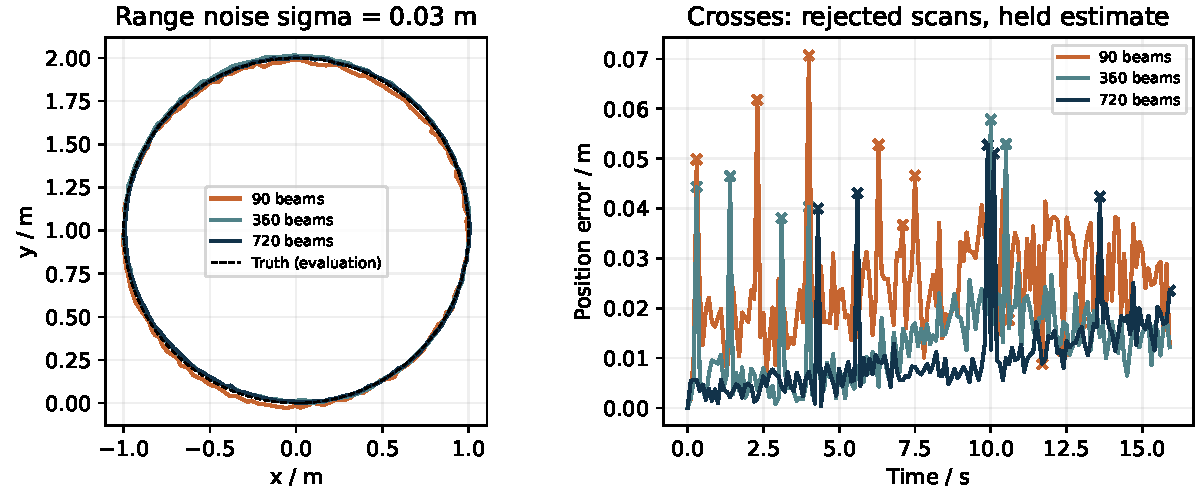
\includegraphics[width=\textwidth]{figures/ch08_odometry.pdf}
\caption{首帧对齐后的轨迹与位置误差。叉号是拒绝帧，此时画出保持上次估计的误差；圆轨迹保持等比例。}
\end{figure}

默认 ROS 实验的 0 到 3 s 共 31 次扫描中，30 次成功、1 次拒绝，
成功帧最大位置误差约 0.00214 m。这是一个固定种子小场景，不能推广为普遍精度承诺。
教材的六组回放也没有在配准后用真值修正结果。720 束不保证每项指标都优于 360 束：
法向量、关联和噪声共同影响局部优化。

\textbf{本章验收：}核心测试覆盖独立差分、恢复、退化、缺帧和有限窗口；
实际 ROS 核对输入隔离、采样时刻、点云/地图、暂停与重播。
继续实验时，一次只改一个参数，记录成功率、误差及失败状态。
下一章使用原始 IMU 预测和激光校正，在同一时间轴上估计速度与偏置。
